%% This file is a portion of the source for Revised Edition 1.1 of
%% Operating Systems and Middleware: Supporting Controlled
%% Interaction, Copyright 2011 by Max Hailperin.  This work is
%% licensed under the Creative Commons Attribution-ShareAlike 3.0
%% Unported License. To view a copy of this license, visit
%% http://creativecommons.org/licenses/by-sa/3.0/ or send a letter to
%% Creative Commons, 171 Second Street, Suite 300, San Francisco,
%% California, 94105, USA.
\chapter{Scheduling}
\label{scheduling-chapter}
\section{Introduction}
In Chapter~\ref{threads-chapter} you saw that operating systems support the concurrent execution
of multiple threads by repeatedly switching each processor's attention
from one thread to another.  This switching implies that some mechanism, known
as a \vocab{scheduler}, is needed to choose which thread to run at each time.
Other system resources may need scheduling as well; for example, if
several threads read from the same disk drive, a disk
scheduler may place them in order.  For simplicity, I will consider
only processor scheduling.  Normally, when people speak of
\vocab{scheduling}, they mean processor scheduling;
similarly, the \vocab{scheduler} is understood to mean the processor
scheduler.

A scheduler should make decisions in a way that keeps the computer
system's users happy.  For example, picking the same thread all the
time and completely ignoring the others would generally not be a good
scheduling policy.  Unfortunately, there is no one policy that will
make all users happy all the time.  Sometimes the reason is as simple as
different users having conflicting desires: for example, user A wants
task A completed quickly, while user B wants task B completed quickly.
Other times, though, the relative merits of different scheduling
policies will depend not on whom you ask, but rather on the context in
which you ask.  As a simple example, a student enrolled in several
courses is unlikely to decide which assignment to work on without
considering when the assignments are due.

Because scheduling policies need to respond to context, operating
systems provide scheduling
mechanisms that leave the user in charge of more subtle policy
choices.  For example, an operating system may provide a mechanism for
running whichever thread has the highest numerical priority, while
leaving the user the job of assigning priorities to the threads.  Even
so, no one mechanism (or general family of policies) will suit all
goals.  Therefore, I spend much of this chapter describing the
different goals that users have for schedulers and the mechanisms that
can be used to achieve those goals, at least approximately.
Particularly since users may wish to achieve several conflicting
goals, they will generally have to be satisfied with ``good enough.''

Before I get into the heavily values-laden scheduling issues, though,
I will present one goal everyone can agree upon:  A thread that can
make productive use of a processor should always be preferred over one
that is waiting for something, such as the completion of a time delay
or the arrival of input.  In Section~\ref{thread-states-section}, you will see how
schedulers arrange for this by keeping track of each thread's state
and scheduling only those that can run usefully.

Following the section on thread states, I devote Section~\ref{scheduling-goals-section} entirely
to the question of users' goals, independent of how they are realized.
Then I spend one section apiece on three broad families of
schedulers, examining for each not only how it works but also how it
can serve users' goals.  These three families of schedulers are those
based on fixed thread priorities (Section~\ref{fixed-priority-scheduling-section}), those based on dynamically adjusted
thread priorities (Section~\ref{dynamic-priority-scheduling-section}), and those based less on priorities than on
controlling each thread's proportional share of processing time (Section~\ref{proportional-share-scheduling-section}).  This three-way division
is not the only possible taxonomy of schedulers, but it will serve to
help me introduce several operating systems' schedulers and
explain the principles behind them while keeping in mind the context
of users' goals.  After presenting the three families of schedulers, I
will briefly remark in Section~\ref{scheduling-security-section} on the role scheduling plays in system security.  The chapter concludes
with exercises,
programming and exploration projects, and notes.

\section{Thread States}\label{thread-states-section}
A typical thread will have times when it is waiting for some event,
unable to execute any useful instructions until the event occurs.
Consider a web server that reads a client's
request from the network, reads the requested web page from disk, and
then sends the page over the network to the client.  Initially the
server thread is waiting for the network interface to have some data
available.  If the server thread were scheduled on a processor while
it was waiting, the best it could do would be to execute a loop that
checked over and over whether any data has arrived---hardly a
productive use of the processor's time.  Once data is available from
the network, the server thread can execute some useful instructions to
read the bytes in and check whether the request is complete.  If not,
the server needs to go back to waiting for more data to arrive.  Once the
request is complete, the server will know what page to load from disk
and can issue the appropriate request to the disk drive.  At that
point, the thread once again needs to wait until such time as the
disk has completed the requisite physical movements to locate the
page.  To take a different example, a video display program may
display one frame of video and then wait some fraction of a second
before displaying the next so that the movie doesn't play too fast.
All the thread could do between frames would be to keep checking
the computer's real-time clock to see whether enough time had
elapsed---again, not a productive use of the processor.

In a single-thread system, it is plausible to wait by executing a loop
that continually checks for the event in question.  This approach is
known as \foldvocab{busy}{waiting}.  However, a modern general-purpose operating
system will have multiple threads competing for the processor.  In
this case, busy waiting is a bad idea because any time that the
scheduler allocates to the busy-waiting thread is lost to the other
threads without achieving any added value for the thread that is
waiting.

Therefore, operating systems provide an alternative way for threads to
wait.
The operating system keeps track of which threads can usefully run
and which are waiting.  The system does this by storing runnable threads in a
data structure called the \vocab{run queue} and waiting threads in
\vocabs{wait queue}, one per reason for waiting.  Although these
structures are conventionally called queues, they may not be used in
the first-in, first-out style of true queues.
For example, there may be a list of threads waiting for time to elapse, kept in order
of the desired time.  Another example of a wait queue would be a set of threads waiting for the
availability of data on a particular network communication channel.

Rather than executing a busy-waiting loop, a thread that wants
to wait for some event notifies the operating system of this intention.  The operating
system removes the thread from the
run queue and inserts the thread into the appropriate wait queue, as shown in
Figure~\ref{scan-3-1}.
\begin{figure}
\centerline{\includegraphics{hail_f0301}}
\caption{When a thread needs to wait, the operating system moves it
  from the run queue to a wait queue.  The scheduler selects one of
  the threads remaining in the run queue to dispatch, so it starts
  running.}
\label{scan-3-1}
\end{figure}
Because the
scheduler considers only threads in the run queue for execution, it
will never select
the waiting thread to run. The scheduler will be choosing only from
those threads that can make progress if given a processor on which to run.

In Chapter~\ref{threads-chapter}, I mentioned that the arrival of a hardware
interrupt can cause the processor to temporarily stop executing
instructions from the current thread and to start executing instructions
from the operating system's interrupt handler.  One of the services this
interrupt handler can perform is determining that a waiting thread doesn't
need to wait any longer.  For example, the computer's real-time clock
may be configured to interrupt the processor every one hundredth of a
second.  The interrupt handler could check the first thread in the
wait queue of threads that are waiting for specific times to elapse.  If the time
this thread was waiting for has not yet arrived, no further threads
need to be checked because the threads are kept in time order.  If,
on the other hand, the thread has slept as long as it requested, then
the operating system can move it out of the list of sleeping threads
and into the run queue, where the thread is available for scheduling.  In
this case, the operating system should check the next thread
similarly, as illustrated in Figure~\ref{scan-3-5}.
\begin{figure}
\centerline{\includegraphics{hail_f0302}}
\caption{When the operating system handles a timer interrupt, all
  threads waiting for times that have now past are moved to the run
  queue. Because the wait queue is kept in time order, the scheduler
  need only check threads until it finds one waiting for a time still
  in the future. In this figure, times are shown on a human scale for
  ease of understanding.}
\label{scan-3-5}
\end{figure}

Putting together the preceding information, there are at least
three distinct states a thread can be in:
\begin{itemize}
\item \vocabindex{Runnable}{runnable} (but not running), awaiting dispatch by the scheduler
\item \vocabindex{Running}{running} on a processor
\item \vocabindex{Waiting}{waiting} for some event
\end{itemize}
Some operating systems may add a few more states in order to make
finer distinctions (waiting for one kind of event versus waiting for
another kind) or to handle special circumstances (for example, a thread that
has finished running, but needs to be kept around until another thread
is notified).  For simplicity, I will stick to the three basic states
in the foregoing list.  At critical moments in the thread's lifetime, the
operating system will change the thread's state.  These thread state
changes are indicated in Figure~\ref{state-diagram}. Again, a real
operating system may add a few additional transitions; for example, it
may be possible to forcibly terminate a thread, even while it is in a
waiting state, rather than having it terminate only of its own accord
while running.
\begin{figure}
\centerline{\includegraphics{hail_f0303}}
\caption{Threads change states as shown here. When a thread is initially created, it is runnable, but not
  actually running on a processor until dispatched by the scheduler.
  A running thread can voluntarily yield the processor or can be preempted
  by the scheduler in order to run another thread.  In either case,
  the formerly running thread returns to the runnable state.
  Alternatively, a running thread may wait for an external event before becoming runnable again. A running thread may also terminate.}
\label{state-diagram}
\end{figure}

\section{Scheduling Goals}\label{scheduling-goals-section}

Users expect a scheduler to maximize the computer system's
performance and to allow them to exert control.  Each of these goals
can be refined into several more precise goals, which I explain in the
following subsections.  High performance may mean high throughput
(Section~\ref{throughput-section}) or fast response time
(Section~\ref{response-time-section}), and user control may be
expressed in terms of urgency, importance, or resource allocation
(Section~\ref{uira-section}).

\subsection{Throughput}\label{throughput-section}
Many personal computers have far more processing capability available
than work to do, and they largely sit idle, patiently waiting for the next
keystroke from a user.  However, if you look behind the scenes at a large
Internet service, such as Google, you'll see a very different
situation.  Large rooms filled with rack after rack of
computers are necessary in order to keep up with the pace of incoming
requests; any one computer can cope only with a small fraction of the
traffic.  For economic reasons, the service provider wants to keep the
cluster of servers as small as possible.  Therefore, the throughput of
each server must be as high as possible.  The \vocab{throughput} is the rate
at which useful work, such as search transactions, is accomplished.
An example measure of throughput would be the number of search
transactions completed per second.

Maximizing throughput certainly implies that the scheduler should give
each processor a runnable thread on which to work, if at all possible.
However, there are some other, slightly less obvious, implications as
well.  Remember that a computer system has more components than just
processors.  It also has I/O devices (such as disk drives and network
interfaces) and a memory hierarchy, including cache memories.  Only by
using all these resources efficiently can a scheduler maximize
throughput.

I already mentioned I/O devices in Chapter~\ref{threads-chapter}, with the
example of a computationally intensive graphics rendering program
running concurrently with a disk-intensive virus scanner.  I will return
to this example later in the current chapter to see one way in which
the two threads can be efficiently interleaved.  In a nutshell, the
goal is to keep both the processor and the disk drive busy all the
time.  If you have ever had an assistant for a project, you may have some
appreciation for what this entails: whenever your assistant was in danger
of falling idle, you had to set your own work aside long enough to
explain the next assignment.  Similarly, the processor must switch
threads when necessary to give the disk more work to do.

Cache memories impact throughput-oriented scheduling in two ways,
though one arises only in \index{multiprocessor system}multiprocessor systems.  In any system,
switching between different threads more often than necessary will
reduce throughput because processor time will be wasted on the
overhead of context switching, rather than be available for useful
work.  The main source of this context-switching overhead is not the
direct cost of the switch itself, which entails saving a few registers out and
loading them with the other thread's values.  Instead, the big cost is
in reduced cache memory performance, for reasons I will explain in a
moment.  On multiprocessor systems a second issue arises:
a thread is likely to run faster when scheduled on the same
processor as it last ran on.  Again, this results from cache memory effects.  To
maximize throughput, schedulers therefore try to maintain
a specific \foldvocab{processor}{affinity} for each thread,
that is, to consistently schedule the thread on the same processor
unless there are
other countervailing considerations.

You probably learned in a computer organization course that
\vocabyies{cache memor} provide fast storage for those addresses that have been
recently accessed or that are near to recently accessed locations.
Because programs frequently access the same locations again (that is,
exhibit \foldvocab{temporal}{locality}) or access nearby locations
(that is, exhibit
\foldvocab{spatial}{locality}), the processor will often be able to get its data
from the cache rather than from the slower main memory.  Now
suppose the processor switches threads.  The new thread will have its own favorite
memory locations, which are likely to be quite different.  The cache
memory will initially suffer many misses, slowing the processor to the
speed of the main memory, as shown in Figure~\ref{scan-3-2}.
\begin{figure}
\centerline{\includegraphics{hail_f0304}}
\caption{When a processor has been executing thread A for a while, the
  cache will mostly hold thread A's values, and the cache hit rate may
  be high.  If the processor then
  switches to thread B, most memory accesses will miss in the cache
  and go to the slower main memory.}
\label{scan-3-2}
\end{figure}
Over time, however, the new thread's data
will displace the data from the old thread, and the performance will
improve.  Suppose that just at the point where the cache has adapted to
the second thread, the scheduler were to decide to
switch back.  Clearly this is not a recipe for high-throughput
computing.

On a multiprocessor system, processor affinity improves throughput in
a similar manner by reducing the number of cycles the processor
stalls waiting for data from slower parts of the memory hierarchy.
Each processor has its own local cache
memory.  If a thread resumes running on the same processor on which it
previously ran, there is some hope it will find its data still in
the cache.  At worst, the thread will incur cache misses and need to
fetch the data from main memory.  The phrase ``at worst'' may seem odd
in the context of needing to go all the way to main memory, but in a
multiprocessor system, fetching from main memory is not the highest
cost situation.

Memory accesses are even more expensive if they refer
to data held in another processor's cache.  That situation can easily
arise if the thread is dispatched on a different processor than it
previously ran on, as shown in Figure~\ref{scan-3-3}
\begin{figure}
\centerline{\includegraphics{hail_f0305}}
\caption{If processor 1 executes thread A and processor 2 executes
  thread B, after a while each cache will hold the corresponding
  thread's values.  If the scheduler later
  schedules each thread on the opposite processor, most
  memory accesses will miss in the local cache and need to use the
  cache coherence protocol to retrieve data from the other cache.}
\label{scan-3-3}
\end{figure}
In this circumstance, the multiprocessor system's
\foldvocab{cache}{coherence protocol} comes into play.  Typically, this means first
transferring the data from the old cache to the main memory and then
transferring it from the main memory to the new cache.  This excess
coherence traffic (beyond what is needed for blocks shared by multiple
threads) reduces throughput if the scheduler has not arranged for
processor affinity.

\subsection{Response Time}\label{response-time-section}

Other than throughput, the principle measure of a computer system's
performance is \vocab{response time}: the elapsed time from a triggering event (such as
a keystroke or a network packet's arrival) to the completed response
(such as an updated display or the transmission of a reply packet).
Notice that a high-performance system in one sense may be
low-performance in the other.  For example, frequent context switches,
which are bad for throughput, may be necessary to optimize
response time.  Systems intended for direct interaction with a single
user tend to be optimized for response time, even at the expense of
throughput, whereas centralized servers are usually designed for high
throughput as long as the response time is kept tolerable.

If an operating system is trying to schedule more than one runnable thread
per processor and if each thread is necessary in order to
respond to some event, then response time inevitably involves
tradeoffs.  Responding more quickly to one event by running the
corresponding thread means responding more slowly to some other event
by leaving its thread in the runnable state, awaiting later
dispatch.  One way to resolve this trade-off is by using
user-specified information on the relative urgency or importance of
the threads, as I describe in Section~\ref{uira-section}.  However, even without that
information, the operating system may be able to do better than just
shrug its virtual shoulders.

Consider a real world situation.  You get an email from a long-lost
friend, reporting what has transpired in her life and asking for a
corresponding update on what you have been doing for the last several
years.  You have barely started writing what will inevitably be a long
reply when a second email message arives, from a close friend, asking
whether you want to go out tonight.  You have two choices.  One is to
finish writing the long letter and then reply ``sure'' to the second
email.  The other choice is to temporarily put your long letter aside,
send off the one-word reply regarding tonight, and then go back to
telling the story of your life.  Either choice extends your response
time for one email in order to keep your response time for the other
email as short as possible.  However, that symmetry doesn't mean there is no logical
basis for choice.  Prioritizing the one-word reply provides much more
benefit to its response time than it inflicts harm on the other, more
time-consuming task.

If an operating system knows how much processor time each thread will
need in order to respond, it can use the same logic as in the email
example to guide its choices.  The policy of \vocab{Shortest Job
First} (\vocab{SJF}) scheduling minimizes the average response time,
as you can demonstrate in Exercise~\ref{Gantt-SJF-exercise}.
This policy dates back to \vocab{batch processing} systems, which processed a
single large \vocab{job} of work at a time, such as a company's
payroll or accounts payable.  System operators could minimize the
average \vocab{turnaround time} from when a job was submitted until it
was completed by processing the shortest one first.  The operators
usually had a pretty good idea how long each job would take, because
the same jobs were run on a regular basis.  However, the reason why
you should be interested in SJF is not for scheduling batch jobs
(which you are unlikely to encounter), but as background for
understanding how a modern operating system can improve the
responsiveness of threads.

Normally an operating system won't know how much processor time each
thread will need in order to respond.  One solution is to guess, based
on past behavior.  The system can prioritize those threads that have not consumed
large bursts of processor time in the past, where a \vocab{burst} is
the amount of processing done between waits for external events.
Another solution is for
the operating system to hedge its bets, so that that even if it
doesn't know which thread needs to run only briefly, it won't sink too
much time into the wrong thread.  By switching frequently between the
runnable threads, if any one of them needs only a little processing time,
it will get that time relatively soon even if the other threads
involve long computations.

The succesfulness of this hedge depends not only on the duration of
the \vocabs{time slice} given to the threads, but also on the number of runnable
threads competing for the processor.  On a lightly loaded system,
frequent switches may suffice to ensure responsiveness.  By contrast,
consider a system that is heavily loaded with many long-running
computations, but that also occasionally has an interactive thread that
needs just a little processor time.  The operating system can 
ensure responsiveness only by identifying and prioritizing the interactive
thread, so that it doesn't have to wait in line behind all the other
threads' time slices.  However brief each of those time slices is, if
there are many of them, they will add up to a substantial delay.

\subsection{Urgency, Importance, and Resource Allocation}\label{uira-section}

The goals of high throughput and quick response time do not inherently
involve user control over the scheduler; a sufficiently smart
scheduler might make all the right decisions on its own.  On the other
hand, there are user goals that revolve precisely around the desire to
be able to say the following: ``{\em This} thread is a high priority; work on it.''
I will explain three different notions that often get
confusingly lumped under the heading of priority.  To disentangle
the confusion, I will use different names for each of
them: \vocab{urgency}, \vocab{importance}, and \foldvocab{resource}{allocation}.  I will reserve
the word \vocab{priority} for my later descriptions of specific
scheduling mechanisms, where it may be used to help achieve any of the
goals: throughput, responsiveness, or the control of urgency, importance,
or resource allocation.

A task is urgent if it needs to be done soon.  For example, if you
have a small homework assignment due tomorrow and a massive term
paper to write within the next two days, the homework is more urgent.
That doesn't necessarily mean it would be smart for you to prioritize
the homework; you might make a decision to take a zero on the homework
in order to free up more time for the term paper.  If so, you are
basing your decision not only on the two tasks' urgency, but also on
their importance; the term paper is more important.  In other words,
importance indicates how much is at stake in accomplishing a task in
a timely fashion.

Importance alone is not enough to make good scheduling decisions
either.  Suppose the term paper wasn't due until a week from now.  In
that case, you might decide to work on the homework today, knowing
that you would have time to write the paper starting tomorrow.  Or, to
take a third example, suppose the term paper (which you have yet to
even start researching) was due in an hour, with absolutely no late
papers accepted.  In that case, you might realize it was hopeless to
even start the term paper, and so decide to put your time into the
homework instead.

Although urgency and importance are quite different matters, the
precision with which a user specifies urgency will determine how that
user can control scheduling to reflect importance.  If tasks have
hard deadlines, then importance can be dealt with as in the
homework example---through a process of ruthless triage.  Here,
importance measures the cost of dropping a task entirely.  On the
other hand, the deadlines may be ``soft,'' with the importance
measuring how bad it is for each task to be late.  At the other
extreme, the user might provide no information at all about urgency,
instead demanding all results ``as soon as possible.''  In this case,
a high importance task might be one to work on whenever possible,
and a low importance task might be one to fill in the idle moments,
when there is nothing more important to do.

Other than urgency and importance, another way in which users may wish to express the relationship
between different threads is by controlling what fraction of the available
processing resources they are allocated.  Sometimes, this is a matter
of fairness.  For example, if two users are sharing a computer, it
might be fair to devote half of the processing time to one user's
threads and the other half of the processing time to the other user's
threads.  In other situations, a specific degree of inequity may be
desired.  For example, a web hosting company may
sell shares of a large server to small companies for their web sites.
A company that wants to provide good service to a growing customer
base might choose to buy two shares of the web server, expecting to
get twice as much of the server's processing time in return for a
larger monthly fee.

When it was common for thousands of users, such as university
students, to share a single computer, considerable attention was
devoted to so-called \foldvocab{fair-share}{scheduling}, in which users'
consumption of the shared processor's time was balanced out over
relatively long time periods, such as a week.  That is, a user who did
a lot of computing early in the week might find his threads allocated
only a very small portion of the processor's time later in the week,
so that the other users would have a chance to catch up.
A fair share didn't have to mean an equal share; the system
administrator could grant differing allocations to different users.
For example, students taking an advanced course might receive more computing
time than introductory students.

With the advent of personal computers, fair-share scheduling has
fallen out of favor, but another resource-allocation approach,
\foldvocab{proportional-share}{scheduling}, is still very much alive. (For example,
you will see that the Linux scheduler is largely based on the
proportional-share scheduling idea.)  The main reason why I mention
fair-share scheduling is to distinguish it from proportional-share
scheduling, because the two concepts have names that are so
confusingly close.

Proportional-share scheduling balances the processing time given to
threads over a much shorter time scale, such as a second.  The idea is
to focus only on those threads that are runnable and to allocate
processor time to them in proportion with the shares the user has
specified.  For example, suppose that I have a big server on which
three companies have purchased time.  Company A pays more per month
than companies B and C, so I have given two shares to company A and
only one share each to companies B and C.  Suppose, for simplicity,
that each company runs just one thread, which I will call thread A,
B, or C, correspondingly.  If thread A waits an hour for some input to
arrive over the network while threads B and C are runnable, I will
give half the processing time to each of B and C, because they each have
one share.  When thread A's input finally arrives and the thread
becomes runnable, it won't be given an hour-long block of processing
time to ``catch up'' with the other two threads.  Instead, it will get
half the processor's time, and threads B and C will each get one
quarter, reflecting the 2:1:1 ratio of their shares.

The simplest sort of proportional-share scheduling
allows shares to be specified only for individual threads,
such as threads A, B, and C in the preceding example.
A more sophisticated version
allows shares to be specified collectively for all the threads run by
a particular user or otherwise belonging to a logical group.  For
example, each user might get an equal share of the
processor's time, independent of how many runnable threads the user
has.  Users who run multiple threads simply subdivide their shares of
the processing time.  Similarly, in the example where a big server is
contracted out to multiple companies, I would probably want to allow
each company to run multiple threads while still controlling the
overall resource allocation among the companies, not just among the
individual threads.

Linux's scheduler provides a flexible \foldvocab{group}{scheduling} facility.  Threads can be treated individually or they can be placed into groups either by user or in any other way that the system administrator chooses. Up through version 2.6.37, the default was for threads to receive processor shares individually.  However, this default changed in version 2.6.38.  The new default is to automatically establish a group for each terminal window.  That way, no matter how many CPU-intensive threads are run from within a particular terminal window, they won't greatly degrade the system's overall performance.  (To be completely precise, the automatically created groups correspond not to terminal windows, but to groupings of processes known as sessions.  Normally each terminal window corresponds to a session, but there are also other ways sessions can come into existence.  Sessions are not explained further in this book.)

Having learned about urgency, importance, and resource allocation,
one important lesson is that without further clarification, you cannot
understand what a user means by a sentence such as ``thread A is
higher priority than thread B.''  The user may want you
to devote twice as much processing time to A as to B, because A is
higher priority in the sense of meriting a larger proportion of
resources.  Then again, the user may want you to devote almost all
processing time to A, running B only in the spare moments when A goes
into a waiting state, because A is higher priority in the sense of
greater importance, greater urgency, or both.

Unfortunately, many operating systems have traditionally not given the
user a rich enough vocabulary to directly express more than one of
these goals.  For example, the UNIX family of operating systems
(including Mac OS~X and Linux) provides a way for the user to specify
the \vocab{niceness} of a thread.  The word \vocab{nice} should be understood
in the sense that a very nice thread is one that is prone to saying,
``Oh no, that's all right, you go ahead of me, I can wait.''  In other
words, a high niceness is akin to a low priority.  However, different
members of this operating system family interpret this single
parameter, niceness, differently.

The original tradition, to which Mac OS~X still adheres, is that
niceness is an expression of importance; a very nice thread should
normally only run when there is spare processor time.  Some newer
UNIX-family schedulers, such as in Linux, instead interpret the same
niceness number as an expression of resource allocation proportion,
with nicer threads getting proportionately less processor time.  It is
pointless arguing which of these interpretations of niceness is the
right one; the problem is that users have two different things they
may want to tell the scheduler, and they will never be able to do so with
only one control knob.

Luckily, some operating systems have provided somewhat more expressive
vocabularies for user control.  For example, Mac OS~X allows the user
to either express the urgency of a thread (through a deadline and
related information) or its importance (through a niceness).  These
different classes of threads are placed in a hierarchicial
relationship; the assumption is that all threads with explicit urgency
information are more important than any of the others.  Similarly, some
proportional-share schedulers, including Linux's, use niceness for
proportion control, but also allow threads to be explicitly flagged as
low-importance threads that will receive almost no processing unless a processor is otherwise idle.

As a summary of this section, Figure~\ref{scan-3-6} shows a taxonomy
of the scheduling goals I have described.  Figure~\ref{scan-3-7}
previews the scheduling mechanisms I describe in the next three
sections, and Figure~\ref{scheduling-table} shows which goals each of
them is designed to satisfy.
\begin{figure}
\centerline{\includegraphics{hail_f0306}}
\caption{A user may want the scheduler to improve system
  performance or to allow user control.  Two different performance
  goals are high throughput and fast response time.  Three different
  ways in which a user may exert control are by specifying threads'
  urgency, importance, or resource share.}
\label{scan-3-6}
\end{figure}
\begin{figure}
\centerline{\includegraphics{hail_f0307}}
\caption{A scheduling mechanism may be based on always running the highest
  priority thread, or on pacing the threads to each receive a
  proportional share of processor time.  Priorities may be fixed, or
  they may be adjusted to reflect either the deadline by which a
  thread must finish or the thread's amount of processor usage.}
\label{scan-3-7}
\end{figure}
\begin{figure}
\centerline{\begin{tabular}{|c|c|}
\hline
\bf Mechanism & \bf Goals\\\hline
fixed priority & urgency, importance\\
Earliest Deadline First & urgency\\
decay usage & importance, throughput, response time\\
proportional share & resource allocation\\
\hline
\end{tabular}}
\caption{For each scheduling mechanism I present, I explain how it can
satisfy one or more of the scheduling goals.}
\label{scheduling-table}
\end{figure}

\section{Fixed-Priority Scheduling}\label{fixed-priority-scheduling-section}

Many schedulers use a numerical \vocab{priority} for each thread;
this controls which threads are selected for execution.  The threads with
higher priority are selected in preference to those with lower priority.
No thread will ever be running if another thread with higher priority
is not running, but is in the
runnable state.  The simplest
way the priorities can be assigned is for the user to manually specify
the priority of each thread, generally with some default value if none
is explicitly specified.  Although there may be some way for the user
to manually change a thread's priority, one speaks of \foldvocab{fixed-priority}{scheduling}
as long as the operating system never automatically adjusts a
thread's priority.

Fixed-priority scheduling suffices to achieve user goals only under limited
circumstances.  However, it is simple, so many real systems offer it, at least as one option.
For example, both Linux and Microsoft Windows allow fixed-priority
scheduling to be selected for specific threads.  Those threads take
precedence over any others, which are scheduled using other means I
discuss in Sections \ref{decay-usage-scheduling-section} and \ref{proportional-share-scheduling-section}.  In fact, fixed-priority scheduling is
included as a part of the international standard known as POSIX, which
many operating systems attempt to follow.

As an aside about priorities, whether fixed or otherwise, it is
important to note that some real systems use smaller priority numbers
to indicate more preferred threads and larger priority numbers to
indicate those that are less preferred.  Thus, a ``higher priority''
thread  may actually be indicated by a
lower priority number.
In this book, I will consistenty use ``higher priority'' and ``lower
priority'' to mean more and less preferred, independent of how those
are encoded as numbers by a particular system.

In a fixed-priority scheduler, the run queue can be kept in a
data structure ordered by priority.  If you have studied algorithms
and data structures, you know that in theory this could be efficiently
done using a clever representation of a priority queue, such as a
binary heap.  However, in practice, most operating systems use a much
simpler structure, because they use only a small range of integers for
the priorities.  Thus, it suffices to keep an array with one entry per
possible priority.  The first entry contains a list of threads with
the highest priority, the second entry contains a list of threads with
the next highest priority, and so forth.

Whenever a processor becomes idle because a thread has terminated or
entered a waiting state, the scheduler dispatches a runnable thread
of highest available priority.  The scheduler also compares priorities when a thread becomes runnable
because it is newly initiated or because it is done waiting.
If the newly runnable thread has higher priority than a running thread, the scheduler preempts the
running thread of lower priority; that is, the lower-priority thread
ceases to run and returns to the run queue.  In its
place, the scheduler dispatches the newly runnable thread of higher
priority.

Two possible strategies exist for dealing with ties, in which two or more
runnable threads have equally high priority.  (Assume there is only
one processor on which to run them, and that no thread has higher priority
than they do.)  One possibility is to run the thread
that became runnable first until it waits for some event or chooses
to voluntarily yield the processor.  Only then is the second, equally
high-priority thread dispatched. The other possibility is to share the
processor's attention between those threads that are tied for highest
priority by alternating among them in a \vocab{round-robin} fashion.  That
is, each thread runs for some small interval of time (typically tens
or hundreds of milliseconds), and then it is preempted from the clock
interrupt handler and the next thread of equal priority is dispatched,
cycling eventually back to the first of the threads.  The POSIX
standard provides for both of these options; the user can select
either a first in, first out (FIFO) policy or a round robin (RR)
policy.

Fixed-priority scheduling is not viable in an open, general-purpose
environment where a user might accidentally or otherwise create a
high-priority thread that runs for a long time.  However, in an
environment where all the threads are part of a carefully
quality-controlled system design, fixed-priority scheduling may be a
reasonable choice.  In particular, it is frequently used for so-called
\index{real-time system}\vocabs{hard-real-time system}, such as those that control the flaps on
an airplane's wings.

Threads in these hard-real-time systems normally perform periodic
tasks.  For example, one thread may wake up every second to make a
particular adjustment in the flaps and then go back to sleep for the remainder of the
second.  Each of these tasks has a deadline by which it must complete;
if the deadline is missed, the program has failed to meet its
specification.  (That is what is meant by ``hard real time.'')  In the
simplest case, the deadline is the same as the period; for example, each
second's adjustment must be done before the second is up.  The
designers of a system like this know all the threads that will be
running and carefully analyze the ensemble to make sure no deadlines
will ever be missed.  In order to do this, the designers need to have
a worst-case estimate of how long each thread will run, per period.

I can illustrate the analysis of a fixed-priority schedule for a
hard-real-time system with some simple examples, which assume
that the threads are all periodic, with deadlines equal to their
periods, and with no interactions among them other than the
competition for a single processor.  To see how the same general ideas
can be extended to cases where these assumptions don't hold, you could
read a book devoted specifically to real-time systems.

Two key theorems, proved by \index{Liu, C. L.@Liu, C.~L.}Liu and
\index{Layland, James W.}Layland in a 1973 article, make it easy
to analyze such a periodic hard-real-time system under fixed-priority
scheduling:
\begin{itemize}
\item
If the threads will meet their deadlines under any fixed priority
assignment, then they will do so under an assignment that prioritizes
threads with shorter periods over those with longer periods.
This policy is known as
\foldvocab{rate-monotonic}{scheduling}.
\item
To check that deadlines are met, it suffices to consider the worst-case situation, which is that all the threads' periods start at the
same moment.
\end{itemize}
Therefore, to test whether any fixed-priority schedule is feasible,
assign priorities in the rate-monotic fashion.  Assume all the threads
are newly runnable at time 0 and plot out what happens after
that, seeing whether any deadline is missed.

To test the feasibility of a real-time schedule, it is conventional to
use a \vocab{Gantt chart}.  This can be
used to see whether a rate-monotonic fixed-priority schedule will work
for a given set of threads.  If not, some scheduling approach other
than fixed priorities may work, or it may be necessary to redesign
using less demanding threads or hardware with more processing power.

A Gantt chart is a bar, representing the passage of time, divided into
regions labeled to show what thread is running during the
corresponding time interval.  For example, the Gantt chart
\[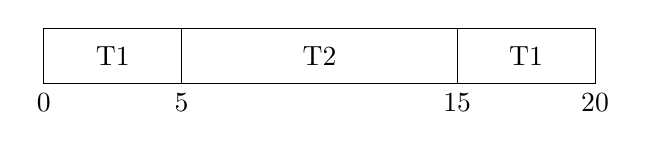
\begin{tikzpicture}[scale=.035]
\draw (0,0) rectangle (50,20);
\draw (50,0) rectangle (150,20);
\draw (150,0) rectangle (200,20);
\draw (25,10) node{T1};
\draw (100,10) node{T2};
\draw (175,10) node{T1};
\draw (0,-7) node{0};
\draw (50,-7) node{5};
\draw (150,-7) node{15};
\draw (200,-7) node{20};
\end{tikzpicture}\]
\iffalse
\[\begin{graph}(210,32)(-3,-12)
\graphlinecolour{0}
\fillednodesfalse
\rectnode{a}[50,20](25,10)
\rectnode{b}[100,20](100,10)
\rectnode{c}[50,20](175,10)
\autonodetext{a}{T1}
\autonodetext{b}{T2}
\autonodetext{c}{T1}
\freetext(0,-7){0}
\freetext(50,-7){5}
\freetext(150,-7){15}
\freetext(200,-7){20}
\end{graph}\]
\fi
\iffalse
\begin{verbatim}
+----+---------+----+
| T1 |    T2   | T1 |
+----+---------+----+
0    5         15   20
\end{verbatim}
\fi
shows thread T1 as running from time 0 to time 5 and again from time
15 to time 20; thread T2 runs from time 5 to time 15.

Consider an example with two periodically executing threads.
One, T1, has a period and deadline of four seconds and a worst-case
execution time per period of two seconds.  The other, T2, has a period
and deadline of six seconds and a worst-case execution time per
period of three seconds.  On the surface, this looks like it might
just barely be feasible on a single processor: T1 has an average
demand of half a processor (two seconds per four) and T2 also has an
average demand of half a processor (three seconds per six), totalling
to one fully utilized, but not oversubscribed, processor.  Assume
that all overheads, such as the time to do context switching between
the threads, have been accounted for by including them in the threads'
worst-case execution times.

However, to see whether this will really work without any missed
deadlines, I need to draw a Gantt chart to determine whether the threads can get the processor when
they need it.  Because T1 has the shorter
period, I assign it the higher priority.  By Liu and Layland's other
theorem, I assume both T1 and T2 are ready to start a period at time
0.  The first six seconds of the resulting Gantt chart looks like this:
\[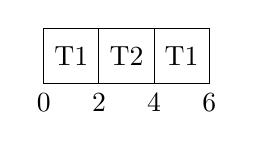
\begin{tikzpicture}[scale=.035]
\draw (0,0) rectangle (20,20);
\draw (20,0) rectangle (40,20);
\draw (40,0) rectangle (60,20);
\draw (10,10) node{T1};
\draw (30,10) node{T2};
\draw (50,10) node{T1};
\draw (0,-7) node{0};
\draw (20,-7) node{2};
\draw (40,-7) node{4};
\draw (60,-7) node{6};
\end{tikzpicture}\]
\iffalse
\[\begin{graph}(70,32)(-3,-12)
\graphlinecolour{0}
\fillednodesfalse
\rectnode{a}[20,20](10,10)
\rectnode{b}[20,20](30,10)
\rectnode{c}[20,20](50,10)
\autonodetext{a}{T1}
\autonodetext{b}{T2}
\autonodetext{c}{T1}
\freetext(0,-7){0}
\freetext(20,-7){2}
\freetext(40,-7){4}
\freetext(60,-7){6}
\end{graph}\]
\fi
\iffalse
\begin{verbatim}
+----+----+----+
| T1 | T2 | T1 |
+----+----+----+
0    2    4    6
\end{verbatim}
\fi
Note that T1 runs initially, when both threads are runnable, because
it has the higher priority.  Thus, it has no difficulty making its
deadline.  When T1 goes into a waiting state at time 2, T2 is able to
start running.  Unfortunately, it can get only two seconds of running
done by the time T1 becomes runnable again, at the start of its second
period, which is time 4.  At that moment, T2 is preempted by the
higher-priority thread T1, which occupies the processor until time 6.
Thus, T2 misses its deadline: by time 6, it has run for only two
seconds, rather than three.

If you accept Liu and Layland's theorem, you will know that switching
to the other fixed-priority assignment (with T2 higher priority than
T1) won't solve this problem.  However, rather than taking this
theorem at face value, you can draw the Gantt chart for
this alternative priority assignment in Exercise~\ref{Gantt-backward-RMS-exercise} and see that again one of the
threads misses its deadline.

In Section~\ref{dynamic-priority-scheduling-section}, I will present a scheduling mechanism
that can handle the preceding scenario successfully.
First, though, I will show one
more example---this time one for which fixed-priority scheduling
suffices.  Suppose T2's worst-case execution time were only two
seconds per six second period, with all other details the same as
before.  In this case, a Gantt chart for the first twelve seconds
would look as follows:
\[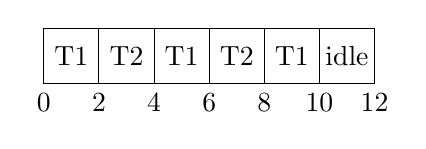
\begin{tikzpicture}[scale=.035]
\draw (0,0) rectangle (20,20);
\draw (20,0) rectangle (40,20);
\draw (40,0) rectangle (60,20);
\draw (60,0) rectangle (80,20);
\draw (80,0) rectangle (100,20);
\draw (100,0) rectangle (120,20);
\draw (10,10) node{T1};
\draw (30,10) node{T2};
\draw (50,10) node{T1};
\draw (70,10) node{T2};
\draw (90,10) node{T1};
\draw (110,10) node{idle};
\draw (0,-7) node{0};
\draw (20,-7) node{2};
\draw (40,-7) node{4};
\draw (60,-7) node{6};
\draw (80,-7) node{8};
\draw (100,-7) node{10};
\draw (120,-7) node{12};
\end{tikzpicture}\]
\iffalse
\[\begin{graph}(130,32)(-3,-12)
\graphlinecolour{0}
\fillednodesfalse
\rectnode{a}[20,20](10,10)
\rectnode{b}[20,20](30,10)
\rectnode{c}[20,20](50,10)
\rectnode{d}[20,20](70,10)
\rectnode{e}[20,20](90,10)
\rectnode{f}[20,20](110,10)
\autonodetext{a}{T1}
\autonodetext{b}{T2}
\autonodetext{c}{T1}
\autonodetext{d}{T2}
\autonodetext{e}{T1}
\autonodetext{f}{idle}
\freetext(0,-7){0}
\freetext(20,-7){2}
\freetext(40,-7){4}
\freetext(60,-7){6}
\freetext(80,-7){8}
\freetext(100,-7){10}
\freetext(120,-7){12}
\end{graph}\]
\fi
\iffalse
\begin{verbatim}
+----+----+----+----+----+----+
| T1 | T2 | T1 | T2 | T1 |idle|
+----+----+----+----+----+----+
0    2    4    6    8    10   12
\end{verbatim}
\fi
Notice that T1 has managed to execute for two seconds during each of
its three periods (0--4, 4--8, and 8--12), and that T2 has managed to
execute for two seconds during each of its two periods (0--6 and 6--12).
Thus, neither missed any deadlines.  Also, you should be able to
convince yourself that you don't need to look any further down the
timeline, because the pattern of the first 12 seconds will repeat
itself during each subsequent 12 seconds.

\section{Dynamic-Priority Scheduling}\label{dynamic-priority-scheduling-section}
Priority-based scheduling can be made more flexible by allowing the
operating system to automatically adjust threads' priorities to
reflect changing circumstances.  The relevant circumstances, and the
appropriate adjustments to make, depend what user goals the system is
trying to achieve.  In this section, I will present a couple different
variations on the theme of dynamically adjusted priorities.  First, for
continuity with Section~\ref{fixed-priority-scheduling-section},
Section~\ref{EDF-section} shows how priorities can
be dynamically adjusted for periodic hard-real-time threads using a
technique known as Earliest Deadline First scheduling.  Then
Section~\ref{decay-usage-scheduling-section} explains decay usage
scheduling, a dynamic adjustment policy commonly used in
general-purpose computing environments.

\subsection{Earliest Deadline First Scheduling}\label{EDF-section}
You saw in Section~\ref{fixed-priority-scheduling-section} that rate-monotonic scheduling is the
optimal fixed-priority scheduling method, but that even it couldn't
schedule two threads, one of which needed two seconds every four and
the other of which needed three seconds every six.  That goal is achievable
with an optimal method for dynamically assigning priorities to
threads.  This method is known as \vocab{Earliest Deadline First} (\vocab{EDF}).  In EDF scheduling,
each time a thread becomes runnable you re-assign priorities
according to the following rule: the sooner a thread's next deadline,
the higher its priority.  The optimality of EDF is another of \index{Liu, C. L.@Liu, C.~L.}Liu and
\index{Layland, James W.}Layland's theorems.

Consider again the example with T1 needing two seconds per four and T2 needing three
seconds per six.
Using EDF scheduling, the Gantt chart for the first twelve seconds of
execution would be as follows:
\[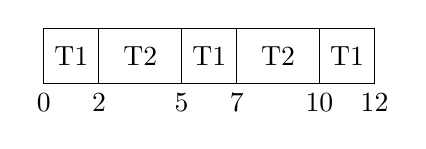
\begin{tikzpicture}[scale=.035]
\draw (0,0) rectangle (20,20);
\draw (20,0) rectangle (50,20);
\draw (50,0) rectangle (70,20);
\draw (70,0) rectangle (100,20);
\draw (100,0) rectangle (120,20);
\draw (10,10) node{T1};
\draw (35,10) node{T2};
\draw (60,10) node{T1};
\draw (85,10) node{T2};
\draw (110,10) node{T1};
\draw (0,-7) node{0};
\draw (20,-7) node{2};
\draw (50,-7) node{5};
\draw (70,-7) node{7};
\draw (100,-7) node{10};
\draw (120,-7) node{12};
\end{tikzpicture}\]
\iffalse
\[\begin{graph}(130,32)(-3,-12)
\graphlinecolour{0}
\fillednodesfalse
\rectnode{a}[20,20](10,10)
\rectnode{b}[30,20](35,10)
\rectnode{c}[20,20](60,10)
\rectnode{d}[30,20](85,10)
\rectnode{e}[20,20](110,10)
\autonodetext{a}{T1}
\autonodetext{b}{T2}
\autonodetext{c}{T1}
\autonodetext{d}{T2}
\autonodetext{e}{T1}
\freetext(0,-7){0}
\freetext(20,-7){2}
\freetext(50,-7){5}
\freetext(70,-7){7}
\freetext(100,-7){10}
\freetext(120,-7){12}
\end{graph}\]
\fi
\iffalse
\begin{verbatim}
+----+-----+----+-----+----+
| T1 | T2  | T1 | T2  | T1 |
+----+-----+----+-----+----+
0    2     5    7     10   12
\end{verbatim}
\fi
There is no need to continue the Gantt chart any further because it
will start repeating.  Notice that neither thread misses any
deadlines: T1 receives two seconds of processor time in each period
(0--4, 4--8, and 8--12), while T2 receives three seconds of processing in
each of its periods (0--6 and 6--12).  This works better
than rate-monotonic scheduling because the threads are prioritized
differently at different times.  At time 0, T1 is prioritized over T2
because its deadline is sooner (time 4 versus 6).  However, when T1
becomes runnable a second time, at time 4, it gets lower priority than
T2 because now it has a later deadline (time 8 versus 6).  Thus, the processor
finishes work on the first period of T2's work, rather than starting in
on the second period of T1's work.

In this example, there is a tie in priorities at time 8, when T1
becomes runnable for the third time.  Its deadline of 12 is the same
as T2's.  If you break the priority tie in favor of the
already-running thread, T2, you obtain the preceding Gantt chart.  In
practice, this is the correct way to break the tie, because it will result
in fewer context switches.  However, in a theoretical sense, any
tie-breaking strategy will work equally well.  In Exercise~\ref{Gantt-EDF-exercise}, you can
redraw the Gantt chart on the assumption that T2 is preempted in order
to run T1.

\subsection{Decay Usage Scheduling}\label{decay-usage-scheduling-section}
Although we all benefit from real-time control systems, such as those
keeping airplanes in which we ride from crashing, they aren't the most
prominent computers in our lives.  Instead, we mostly notice the
workstation computers that we use for daily chores, like typing this
book.  These computers may execute a few real-time threads for tasks
such as keeping an MP3 file of music decoding and playing at its
natural rate.  However, typically, most of the computer user's goals
are not expressed in terms of deadlines, but rather in terms of a
desire for quick response to interaction and efficient (high
throughput) processing of major, long-running computations.  Dynamic
priority adjustment can help with these goals too, in operating
systems such as Mac OS~X or Microsoft Windows.

Occasionally, users of general-purpose workstation computers want to
express an opinion about the priority of certain threads in order to
achieve goals related to urgency, importance, or resource allocation.
This works especially well for importance; for example, a search for
signs of extra-terrestrial intelligence might be rated a low priority
based on its small chance of success.   These
user-specified priorities can serve as \foldvocabyies{base}{priorit}, which the operating
system will use as a starting point for its automatic adjustments.
Most of the time, users will accept the default base priority for all
their threads, and so the only reason threads will differ in priority
is because of the automatic adjustments.  For simplicity, in the
subsequent discussion, I will assume that all threads have the same base
priority.

In this kind of system, threads that tie for top priority after
incorporating the automatic adjustments are processed in a
\index{round-robin}round-robin fashion, as discussed earlier.  That is, each gets to run
for one \vocab{time slice}, and then the scheduler switches
to the next of the threads.
The length of time each thread is allowed to run before switching may
also be called a \vocab{quantum}, rather than a time slice.
The thread need not run for
its full time slice; it could, for example, make an I/O request and go
into a waiting state long before the time slice is up.  In this case,
the scheduler would immediately switch to the next thread.

One reason for the operating system to adjust priorities is to
maximize throughput in a situation in which one thread is
processor-bound and another is disk-bound.  For example, in
Chapter~\ref{threads-chapter}, I introduced a scenario where the user is running a
processor-intensive graphics rendering program in one window, while
running a disk-intensive virus scanning program in another window.  As
I indicated there, the operating system can keep both the processor
and the disk busy, resulting in improved throughput relative to using
only one part of the computer system at a time.  While the disk is
working on a read request from the virus scanner, the processor can be
doing some of the graphics rendering.  As soon as the disk transaction
is complete, the scheduler should switch the processor's attention to
the virus scanner.  That way, the virus scanner can quickly look at
the data that was read in and issue its next read request, so that the
disk drive can get back to work without much delay.  The graphics
program will have time enough to run again once the virus scanning
thread is back to waiting for the disk.  In order to achieve this
high-throughput interleaving of threads, the operating system needs to
assign the disk-intensive thread a higher priority than the
processor-intensive one.

Another reason for the operating system to adjust priorities is to
minimize response time in a situation where an interactive thread is
competing with a long-running computationally intensive thread.  For
example, suppose that you are running a program in one window that is
trying to set a new world record for computing digits of $\pi$, while in
another window you are typing a term paper.  During the long pauses
while you rummage through your notes and try to think of what to write
next, you don't mind the processor giving its attention to computing
$\pi$.  But the moment you have an inspiration and start typing, you want
the word processing program to take precedence, so that it can respond
quickly to your keystrokes.  Therefore, the operating system must have
given this word processing thread a higher priority.

Notice that in both these situations, a computationally intensive
thread is competing with a thread that has been unable to use the
processor for a while, either because it was waiting for a disk
transaction to complete or because it was waiting for the user to
press another key.  Therefore, the operating system should adjust
upward the priority of threads that are in the waiting state and
adjust downward the priority of threads that are in the running state.  In a
nutshell, that is what \index{scheduling, decay usage}\vocabindex{decay usage schedulers}{decay usage scheduling}, such as the one in Mac
OS~X, do.  The scheduler in Microsoft Windows also fits the same
general pattern, although it is not strictly a  decay usage
scheduler.  I will discuss both these schedulers in more detail in the
remainder of this section.

A decay usage scheduler, such as in Mac OS~X, adjusts each thread's
priority downward from the base priority by an amount that reflects
recent processor usage by that thread.  (However, there is some cap on
this adjustment; no matter how much the thread has run, its priority
will not sink below some minimum value.)  If the thread has recently
been running a lot, it will have a priority substantially lower than
its base priority.  If the thread has not run for a long time (because
it has been waiting for the user, for example), then its priority will
equal the base priority.  That way, a thread that wakes up after a
long waiting period will take priority over a thread that has been
able to run.

The thread's recent processor usage increases when the thread runs
and \vocabs{decay} when the thread waits, as shown in
Figure~\ref{scan-3-4}.
\begin{figure}
\centerline{\includegraphics{hail_f0309}}
\caption{In a decay usage scheduler, such as Mac OS~X uses, a thread's
  usage increases while it runs and decays exponentially while it
  waits.  This causes the priority to decrease while running and
  increase while waiting.}
\label{scan-3-4}
\end{figure}
When the thread has been
running, its usage increases by adding in the amount of time that it
ran.  When the thread has been waiting, its usage decreases by being
multiplied by some constant every so often; for example, Mac OS~X
multiplies the usage by 5/8, eight times per second.
Rather than continuously updating the usage of every thread, the
system can calculate most of the updates to a particular thread's usage just when its state
changes, as I describe in the next two paragraphs.

The currently running thread has its usage updated whenever it voluntarily yields the
processor, has its time slice end, or faces potential preemption
because another thread comes out of the waiting state.  At these
points, the amount of time the thread has
been running is added to its usage, and its priority is correspondingly lowered.  In
Mac OS~X, the time spent in the running state is scaled by the current
overall load on the system before it is added to the thread's usage.
That way, a thread that runs during a time of high load will have its
priority drop more quickly to give the numerous other
contending threads their chances to run.

When a thread is done spending time in the waiting state, its usage is
adjusted downward to reflect the number of decay periods that have
elapsed.  For example, in Mac OS~X, the usage is multiplied by
$(5/8)^n$, where $n$ is the number of eighths of a second that have
elapsed.  Because this is an exponential decay, even a fraction of a
second of waiting is enough to bring the priority much of the way back
to the base, and after a few seconds of waiting, even a thread that
previously ran a great deal will be back to base priority.  In fact,
Mac OS~X approximates $(5/8)^n$ as 0 for $n \geq 30$, so any thread
that has been waiting for at least 3.75 seconds will be exactly at
base priority.

Microsoft Windows uses a variation on this theme.  Recall that a decay
usage scheduler adjusts the priority downward from the base to reflect
recent running and restores the priority back up toward the base
when the thead waits.  Windows does the reverse: when a thread comes
out of a wait state, it is given an elevated priority, which then
sinks back down toward the base priority as the thread runs.  The net
effect is the same: a thread that has been waiting gets a higher
priority than one that has been running.  The other difference is in
how the specific numerical size of the change is calculated.  When the
thread runs, Windows decreases its priority down to the base in a
linear fashion, as with decay usage scheduling.  However, Windows does
not use exponential decay to boost waiting threads.  Instead, a thread
that has been waiting is given a priority boost that depends on what
it was waiting for: a small boost after waiting for a disk drive, a
larger boost after waiting for input from the keyboard, and so forth.  Because
the larger boosts are associated with the kinds of waiting that
usually take longer, the net effect is broadly similar to what
exponential decay of a usage estimate achieves.

As described in Section~\ref{fixed-priority-scheduling-section}, a
scheduler can store the run queue as an array of thread lists, one per
priority level.  In this case, it can implement priority adjustments
by moving threads from one level to another.  Therefore, the Mac OS~X
and Microsoft Windows schedulers are both considered examples of the
broader class of \vocabs{multilevel feedback queue scheduler}.  The
original multilevel scheduler placed threads into levels primarily
based on the amount of main memory they used.  It also used longer
time slices for the lower priority levels.  Today, the most important
multilevel feedback queue schedulers are those approximating
decay-usage scheduling.

One advantage to decreasing the priority of running processes below
the base, as in Mac OS~X, rather than only down to the base, as in
Microsoft Windows, is that doing so will normally prevent any runnable
thread from being permanently ignored, even if a long-running thread
has a higher base priority.  Of course, a Windows partisan could reply
that if base priorities indicate importance, the less important thread
arguably should be ignored.  However, in practice, totally shutting
out any thread is a bad idea; one reason is the phenomenon of
\foldvocab{priority}{inversion}, which I will explain in Chapter~\ref{synchronization-chapter}.
Therefore, Windows has a small escape hatch: every few seconds, it
temporarily boosts the priority of any thread that is otherwise unable
to get dispatched.

One thing you may notice from the foregoing examples is the tendancy of
magic numbers to crop up in these schedulers.  Why is the usage
decayed by a factor of 5/8, eight times a second, rather than a factor
of 1/2, four times a second?  Why is the time quantum for round-robin
execution 10 milliseconds under one system and 30 milliseconds under
another?  Why does Microsoft Windows boost a thread's priority by six
after waiting for keyboard input, rather than by five or seven?

The answer to all these questions is that system designers have
tuned the numerical parameters in each system's scheduler by trial
and error.  They have done experiments using workloads similar to those
they expect their system to encounter in real use.  Keeping the
workload fixed, the experimenter varies the scheduler parameters and
measures such performance indicators as response time and throughput.
No one set of parameters will optimize all measures of performance for
all workloads.  However, by careful, systematic experimentation,
parameters can be found that are likely to keep most users happy most
of the time.  Sometimes system administrators can adjust one or more
of the parameters to suit the particular needs of their own
installations, as well.

Before leaving decay usage schedulers, it is worth pointing out one
kind of user goal that these schedulers are not very good at
achieving.  Suppose you have two processing-intensive threads and
have decided you would like to devote two-thirds of your processor's
attention to one and one-third to the other.  If other threads start
running, they can get some of the processor's time, but you still want
your first thread to get twice as much processing as any of the other
threads.  In principle, you might be able to achieve this resource
allocation goal under a decay usage scheduler by appropriately
fiddling with the base priorities of the threads.  However, in
practice it is very difficult to come up with appropriate base
priorities to achieve desired processor proportions.  Therefore, if
this kind of goal is important to a system's users, a different form
of scheduler should be used, such as I discuss in Section~\ref{proportional-share-scheduling-section}.

\section{Proportional-Share Scheduling}\label{proportional-share-scheduling-section}
\foldindex{proportional-share}{scheduling}
When resource allocation is a primary user goal, the scheduler needs
to take a somewhat longer-term perspective than the approaches I have
discussed thus far.  Rather than focusing just on which thread is most
important to run at the moment, the scheduler needs to be pacing the
threads, doling out processor time to them at controlled rates.

Researchers have proposed three basic mechanisms for controlling the
rate at which threads are granted processor time:
\begin{itemize}
\item
Each thread can be granted the use of the processor equally often,
just as in a simple round-robin. However, those that have larger
allocations are granted a longer time slice each time around than
those with smaller allocations.  This mechanism is known as \foldvocab{weighted round-robin}{scheduling} (\vocab{WRR}).
\item
A uniform time slice can be used for all threads.  However, those that
have larger allocations can run more often, because the threads with
smaller allocations ``sit out'' some of the rotations through the list
of runnable threads.  Several names are used for this mechanism, depending
on the context and minor variations: \vocab{weighted fair queuing} (\vocab{WFQ}),
\foldvocab{stride}{scheduling}, and \foldvocab{virtual time round-robin}{scheduling} (\vocab{VTRR}).
\item
A uniform time slice can be used for all threads.  However, those with
larger allocations are chosen to run more often (on the average),
because the threads are selected by a lottery with weighted odds,
rather than in any sort of rotation.  This mechanism is called \foldvocab{lottery}{scheduling}.
\end{itemize}

Lottery scheduling is not
terribly practical, because although each thread will get its
appropriate share of processing time over the long run, there may be
significant deviations over the short run. Consider, for example, a
system with two threads, each of which should get half the processing
time.  If the time-slice duration is one twentieth of a second, each
thread should run ten times per second.  Yet one thread might get shut
out for a whole second, risking a major loss of responsiveness, just
by having a string of bad luck.  A coin flipped twenty times per
second all day long may well come up heads twenty times in a row at
some point.  In Programming Project~\ref{Bernoulli-run-project}, you
will calculate the probability and discover that over the course of a
day the chance of one thread or the other going a whole second
without running is actually quite high.
Despite this shortcoming,
lottery scheduling
has received considerable attention in the research
literature.

Turning to the two non-lottery approaches, I can
illustrate the difference between them with an example.  Suppose
three threads (T1, T2, and T3) are to be allocated
resources in the proportions 3:2:1.  Thus, T1 should get half the
processor's time, T2 one-third, and T3 one-sixth.  With
weighted round-robin scheduling, I might
get the following Gantt chart with times in milliseconds:
\[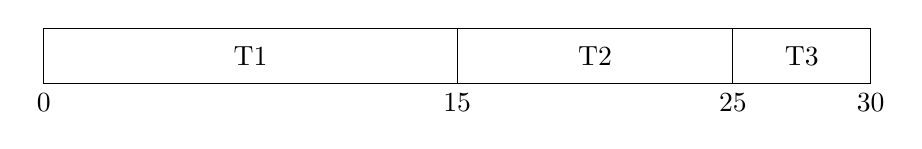
\begin{tikzpicture}[scale=.035]
\draw (0,0) rectangle (150,20);
\draw (150,0) rectangle (250,20);
\draw (250,0) rectangle (300,20);
\draw (75,10) node{T1};
\draw (200,10) node{T2};
\draw (275,10) node{T3};
\draw (0,-7) node{0};
\draw (150,-7) node{15};
\draw (250,-7) node{25};
\draw (300,-7) node{30};
\end{tikzpicture}\]
\iffalse
\[\begin{graph}(310,32)(-3,-12)
\graphlinecolour{0}
\fillednodesfalse
\rectnode{a}[150,20](75,10)
\rectnode{b}[100,20](200,10)
\rectnode{c}[50,20](275,10)
\autonodetext{a}{T1}
\autonodetext{b}{T2}
\autonodetext{c}{T3}
\freetext(0,-7){0}
\freetext(150,-7){150}
\freetext(250,-7){250}
\freetext(300,-7){300}
\end{graph}\]
\fi
Taking the other approach, I could use a fixed time slice of
5~milliseconds, but with T2 sitting out one round in every three, and
T3 sitting out two rounds out of three.  The Gantt chart for the first
three scheduling rounds would look as follows (thereafter, the pattern
would repeat):
\[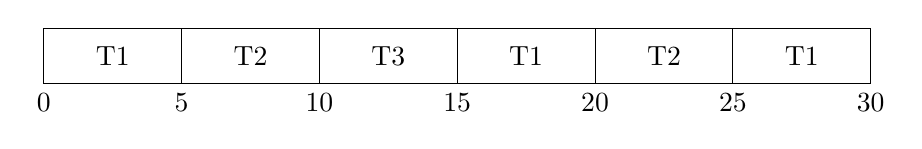
\begin{tikzpicture}[scale=.035]
\draw (0,0) rectangle (50,20);
\draw (50,0) rectangle (100,20);
\draw (100,0) rectangle (150,20);
\draw (150,0) rectangle (200,20);
\draw (200,0) rectangle (250,20);
\draw (250,0) rectangle (300,20);
\draw (25,10) node{T1};
\draw (75,10) node{T2};
\draw (125,10) node{T3};
\draw (175,10) node{T1};
\draw (225,10) node{T2};
\draw (275,10) node{T1};
\draw (0,-7) node{0};
\draw (50,-7) node{5};
\draw (100,-7) node{10};
\draw (150,-7) node{15};
\draw (200,-7) node{20};
\draw (250,-7) node{25};
\draw (300,-7) node{30};
\end{tikzpicture}\]
\iffalse
\[\begin{graph}(310,32)(-3,-12)
\graphlinecolour{0}
\fillednodesfalse
\rectnode{a}[50,20](25,10)
\rectnode{b}[50,20](75,10)
\rectnode{c}[50,20](125,10)
\rectnode{d}[50,20](175,10)
\rectnode{e}[50,20](225,10)
\rectnode{f}[50,20](275,10)
\autonodetext{a}{T1}
\autonodetext{b}{T2}
\autonodetext{c}{T3}
\autonodetext{d}{T1}
\autonodetext{e}{T2}
\autonodetext{f}{T1}
\freetext(0,-7){0}
\freetext(50,-7){50}
\freetext(100,-7){100}
\freetext(150,-7){150}
\freetext(200,-7){200}
\freetext(250,-7){250}
\freetext(300,-7){300}
\end{graph}\]
\fi

Weighted round-robin scheduling has the advantage of fewer thread switches.  Weighted fair queueing, on the other hand, can keep the threads accumulated runtimes more consistently close to the desired proportions.  Exercise~\ref{WRR-WFQ-comparison-exercise} allows you to explore the difference.

In
Linux, the user-specified \vocab{niceness} of a thread controls the
proportion of processor time that the thread will receive.
The core of the scheduling algorithm is a weighted round-robin, as in the first
Gantt chart.
(A separate scheduling policy is used for
fixed-priority scheduling
of real-time threads.  The discussion
here concerns the scheduler  used for
ordinary threads.)
This proportional-share scheduler is called the \vocab{Completely Fair Scheduler} (\vocab{CFS}).
On a multiprocessor system, CFS schedules the threads running on each processor; a largely independent
mechanism balances the overall computational load between processors.  The end-of-chapter notes
revisit the question of how proportional-share scheduling fits into the multiprocessor context.

Rather than directly assign each niceness level a time slice, CFS assigns
each niceness level a \textit{weight} and then calculates the time slices
based on the weights of the runnable threads.  Each thread is given a
time slice proportional to its weight divided by the total weight of
the runnable threads.  CFS starts with a target time for how long it
should take to make one complete round-robin through the runnable
threads.  Suppose, for example, that the target is 6~milliseconds.  Then with
two runnable threads of equal niceness, and hence equal weight, each
thread will run for 3~milliseconds, independent of whether they both have
niceness 0 or both have niceness 19.  With four equal-niceness
threads, each would run 1.5~milliseconds.

Notice that the thread-switching rate is dependent on the overall
system load, unlike with a fixed time slice.  This means that as a
system using CFS becomes more loaded, it will tend to sacrifice some
throughput in order to retain a desired level of responsiveness.  The
level of responsiveness is controlled by the target time that a thread
may wait between successive opportunities to run, which  is settable by the system
administrator.  The value of 6~milliseconds used in the examples is the
default for uniprocessor systems.

However, if system load becomes extremely high, CFS does not
continue sacrificing throughput to response time.  This is because
there is a lower bound on how little time each thread can receive.
After that point is reached, adding additional threads will increase
the total time to cycle through the threads, rather than continuing to
reduce the per-thread time.  The minimum time per thread is also a
parameter the system administrator can configure; the default value
causes the time per thread to stop shrinking once the number of runnable threads reaches 8.

Now consider a case where two threads share the CPU, one with
niceness 0 and the other with niceness 5.  CFS assigns these niceness
levels the weights of 1024 and 335 respectively.  The time that the
threads get is therefore proportional to $1024/(1024+335)$ and
$335/(1024+335)$.  Because 1024 is roughly 3 times as large as 335, we
can estimate that the thread with niceness 0 will receive
approximately 4.5~milliseconds out of each 6~milliseconds and
the thread with niceness 5 will receive approximately 1.5~milliseconds out of each
6~milliseconds.  The same result would be achieved if
the threads had niceness 5 and 10 rather than 0 and 5, because the
weights would then be 335 and 110, which are still in approximately a
3-to-1 ratio.  More generally, the CPU proportion is determined only
by the relative difference in nicenesses, rather than the absolute
niceness levels, because the weights are arranged in a geometric
progression.  (This is analogous to well-tempered musical scales, where a particular
interval, such as a major fifth, has the same harmonic quality no
matter where on the scale it is positioned, because the ratio of
frequencies is the same.)

Having seen this overview of how nicenesses control the allocation of
processor time in CFS, we can now move into a discussion of the actual
mechanism used to meter out the processor time.
The CFS scheduling mechanism is based around one big idea, with
lots of smaller details that I will largely ignore.

The big idea is
keeping track for each thread of how much total running it has done,
measured in units that are scaled in accordance with the thread's
weight.  That is, a niceness 0 thread is credited with 1~nanosecond of running
for each nanosecond of time that elapses with the thread running, but
a niceness 5 thread would be credited with approximately 3~nanoseconds of
running for each nanosecond it actually runs.  (More precisely, it
would be credited with 1024/335 nanoseconds of running for each
actual nanosecond.)

Given this funny accounting of how much running
the threads are doing (which is called \foldvocab{virtual}{runtime}), the goal of keeping the threads running in
their proper proportion simply amounts to running whichever is the
furthest behind.  However, if CFS always devoted the CPU to the thread that was furthest behind,
it would be constantly switching back and forth between the threads.
Instead, the scheduler sticks with the current thread until its
time slice runs out or it is preempted by a waking thread.
Once the scheduler does choose a new thread, it picks the thread
with minimum virtual runtime.  Thus, over the long haul, the virtual
runtimes are kept approximately in balance, which means the actual
runtimes are kept in the proportion specified by the threads'
weights, which reflect the threads'
nicenesses.

This concept of keeping virtual runtimes in balance is important enough
to consider a couple concrete examples.
First, consider a case where two threads have equal niceness, so the scheduler tries to make
sure that the two threads have run for equal amounts of time. After $x$
nanoseconds have elapsed, each of the two threads should have run for $x/2$
nanoseconds.  To make this always exactly true, the scheduler would need to
keep switching back and forth between the threads, which is inefficient.  Instead, the scheduler is willing to stick with one thread for a length of
time, the time slice.  As a result, you might see that after 9~milliseconds,
instead of each of the two threads having run for 4.5~milliseconds, maybe
Thread~A has run for 6~milliseconds and Thread~B has run for 3~milliseconds,
as shown in Figure~\ref{equal-virtual-runtime-figure}.  When the scheduler decides which thread to run next, it
will pick the one that has only run for 3~milliseconds, that is, Thread~B,
so that it has a chance to catch up with Thread~A.  That way, if you check
again later, you won't see Thread~A continuing to get further and further
advantaged over Thread~B.  Instead, you will see the two threads taking
turns for which one has run more, but with the difference between the two of
them never being very large, perhaps 3~milliseconds at most, as this
example suggests.
\begin{figure}
\[\begin{tikzpicture}[scale=.03]
\draw (0,0) rectangle (100,20);
\draw (100,0) rectangle (200,20);
\draw (200,0) rectangle (300,20);
\draw (50,10) node{A};
\draw (150,10) node{B};
\draw (250,10) node{A};
\draw (0,30) node{0};
\draw (100,30) node{3};
\draw (100,37) -- (100,43);
\draw (200,30) node{6};
\draw (200,37) -- (200,43);
\draw (300,30) node{9};
\draw (300,37) -- (300,43);
\draw[->] (0,40) -- (310,40) node[right] {time};
\draw[->] (0,40) -- (0,250) node[above] {virtual runtime};
\draw (0,40) -- (100,140) -- (200,140) -- (300, 240) node[right] {A};
\draw[dashed] (0,40) -- (100,40) -- (200,140) -- (300, 140) node[right] {B};
\draw (-7,140) node{3};
\draw (-3,140) -- (3,140);
\draw (-7,240) node{6};
\draw (-3,240) -- (3,240);
\end{tikzpicture}\]
\caption{Because Thread A and Thread B both have niceness 0, each accumulates 1 millisecond of virtual
runtime for each elapsed millisecond during which it runs.  The bottom of this figure shows a Gantt
chart indicating which thread is running at each point.  The top of the figure plots virtual runtime versus time
for Thread A (solid) and Thread B (dashed). At the 9 millisecond point, the scheduler would choose
Thread B to run next, because it has the lower virtual runtime.}\label{equal-virtual-runtime-figure}
\end{figure}


Now consider what happens when the two threads have different niceness.  For
example, suppose Thread~A has niceness 0 and Thread~B has niceness 5.  To
make the arithmetic easier, let us pretend that $1024/335$ is exactly 3, so
that Thread~A should run exactly 3 times more than Thread~B.  Now, even if
the scheduler did not have to worry about the efficiency problems of
switching between the threads, the ideal situation after 9~milliseconds
would no longer be that each thread has run for 4.5 milliseconds.  Instead,
the ideal would be for Thread~A to have run for 6.75 milliseconds and Thread~B
for only 2.25 milliseconds.  But again, if the scheduler is only switching
threads when discrete time slices expire, this ideal situation will not actually
happen.  Instead, you may see that Thread~A has run for 6~milliseconds and
Thread~B has run for 3~milliseconds, as shown in Figure~\ref{proportional-virtual-runtime-figure}.  Which one should run next?  We can no
longer say that Thread~B is further behind and should be allowed to catch
up.  In fact, Thread~B has run for longer than it ought to have.  (Remember,
it really ought to have only run for 2.25 milliseconds.)  The way the
scheduler figures this out is that it multiplies each thread's time by a
scaling factor.  For Thread~A, that scaling factor is 1, whereas for Thread~B, it is 3.  Thus, although their actual runtimes are 6~milliseconds and
3~milliseconds, their virtual runtimes are 6~milliseconds and 9~milliseconds.  Now, looking at these virtual runtimes, it is clear that
Thread~A  is further behind (it has only 6 virtual milliseconds) and
Thread~B is ahead (it has 9 virtual milliseconds).  Thus, the
scheduler knows to choose Thread~A to run next.
\begin{figure}
\[\begin{tikzpicture}[scale=.03]
\draw (0,0) rectangle (100,20);
\draw (100,0) rectangle (200,20);
\draw (200,0) rectangle (300,20);
\draw (50,10) node{A};
\draw (150,10) node{B};
\draw (250,10) node{A};
\draw (0,30) node{0};
\draw (100,30) node{3};
\draw (100,37) -- (100,43);
\draw (200,30) node{6};
\draw (200,37) -- (200,43);
\draw (300,30) node{9};
\draw (300,37) -- (300,43);
\draw[->] (0,40) -- (310,40) node[right] {time};
\draw[->] (0,40) -- (0,350) node[above] {virtual runtime};
\draw (0,40) -- (100,140) -- (200,140) -- (300, 240) node[right] {A};
\draw[dashed] (0,40) -- (100,40) -- (200,340) -- (300, 340) node[right] {B};
\draw (-7,140) node{3};
\draw (-3,140) -- (3,140);
\draw (-7,240) node{6};
\draw (-3,240) -- (3,240);
\draw (-7,340) node{9};
\draw (-3,340) -- (3,340);
\end{tikzpicture}\]
\caption{Thread A still accumulates 1 millisecond of virtual
runtime for each elapsed millisecond during which it runs, but Thread B accumulates virtual
runtime at approximately 3 times as fast a rate, because it has niceness 5.  The bottom of this figure shows a Gantt
chart indicating which thread is running at each point.  The top of the figure plots virtual runtime versus time
for Thread A (solid) and Thread B (dashed). At the 9 millisecond point, the scheduler would choose
Thread A to run next, because it has the lower virtual runtime, corresponding to the fact that it has
only run twice as much as Thread B, rather than three times as much.
(Assuming both threads remained runnable the whole time, the actual Linux CFS scheduler
would not have given them equal time slices as shown here.  However, the accounting for
virtual runtime works the same in any case.)}\label{proportional-virtual-runtime-figure}
\end{figure}

Notice that if Thread~A and Thread~B in this example were in their ideal
situation of having received 6.75 real milliseconds and 2.25 real milliseconds,
then their virtual runtimes would be exactly tied.  Both threads would
have run for 6.75 virtual milliseconds, once the scaling factors are taken into account.

This description of accumulating virtual runtime would suffice if all
threads started when the system was first booted and stayed
continuously runnable.  However, it needs a bit of
enhancement to deal with threads being created or waking up from timed sleeps and I/O waits.
If the scheduler didn't do anything special with them, they would get
to run until they caught up with the pre-existing threads, which could
be a ridiculous amount of runtime for a newly created thread or one that
has been asleep a long time.  Giving that much runtime to one thread would
deprive all the other threads of their normal opportunity to run.

For a thread that has only been briefly out of the run queue, the CFS actually does allow it to catch up on runtime.  But once a thread has been non-runnable
for more than a threshold amount of time, when it wakes up, its virtual runtime is set forward so as to be only slightly less than the minimum virtual runtime of any of the previously runnable threads.  That way, it will get to run soon but not for much longer than usual.  This is similar to the effect achieved through dynamic priority adjustments in decay usage schedulers and Microsoft Windows.  As with those adjustments, the goal is not proportional sharing, but responsiveness and throughput.

Any newly created thread is given a virtual runtime slightly greater than the minimum virtual runtime of the previously runnable threads, essentially as though it had just run and were now waiting for its next turn to run.

The run queue is kept sorted in order of the runnable threads' virtual runtimes.
The data structure used for this purpose is
a red-black tree, which is a variant of a
binary search tree with the efficiency-enhancing property that no leaf
can ever be more than twice as deep as any other leaf.
When the CFS scheduler decides to switch threads, it switches to the leftmost thread in the
red-black tree, that is, the one with the earliest virtual runtime.

The scheduler performs these thread switches under two
circumstances.  One is the expiration of a time slice.  The other is
when a new thread enters the run queue, provided that the currently
running thread hasn't just recently started running.  (There is a
configurable lower limit on how quickly a thread can be preempted.)

One of the advantages of positioning runnable threads on a timeline
of virtual runtimes (represented as the red-black tree) is that it
naturally prevents waking threads from starving other threads that
have remained runnable, as was possible with earlier Linux schedulers.
As time marches on, threads that wake up get inserted into
the timeline at later and later virtual runtimes.  A runnable thread that has been patiently
waiting for the CPU, on the other hand, retains a fixed virtual runtime.
As such, it will eventually have the lowest virtual runtime, and hence
will be chosen to run (once a thread switch occurs).


\section{Security and Scheduling}\label{scheduling-security-section}

The kind of attack most relevant to
scheduling is the \vocab{denial of service} (\vocab{DoS}) attack, that is, an
attack with the goal of preventing legitimate users of a system from
being able to use it.  Denial of service attacks are frequently
nuisances motivated by little more than the immaturity of the
perpetrators.  However, they can be part of a more sophisticated
scheme.  For example, consider the consequences if a system used for
coordinating a military force were vulnerable to a denial of service
attack.

The most straightforward way an attacker could misuse a scheduler in
order to mount a denial of service attack would be to usurp the
mechanisms provided for administrative control.  Recall that
schedulers typically provide some control parameter for each thread,
such as a deadline, a priority, a base priority, or a resource share.
An authorized system administrator needs to be able to say ``This
thread is a really low priority'' or the analogous statement about
one of the other parameters.  If an attacker could exercise that same
control, a denial of service attack could be as simple as giving a low
priority to a critical thread.

Therefore, real operating systems guard the thread-control interfaces.
Typically, only a user who has been authenticated as the ``owner'' of
a particular thread or as a bona fide system administrator can control
that thread's scheduling parameters.
(Generally the owner of a thread will be whatever user ran the program
that created the thread.)
Naturally, this relies upon
other aspects of the system's security that I will consider in later
chapters: the system must be protected from tampering, must be able to
authenticate the identity of its users, and must be programmed in a
sufficiently error-free fashion that its checks cannot be evaded.

Because real systems guard against an unauthorized user
de-prioritizing a thread, attackers use a slightly more sophisticated
strategy.  Rather than de-prioritizing the targeted thread, they
compete with it.  That is, the attackers create other threads that
attempt to siphon off enough of a scarce resource, such as processor
time, so that little or none will be left for the targeted thread.

One response of system designers has been to arrange that any denial
of service attack will be sufficiently cumbersome that it can be
easily distinguished from normal behavior and hence interdicted.  For
example, recall that a single thread at a high fixed priority could
completely starve all the normal threads.  Therefore, most systems
prohibit normal users from running such threads, reserving that
privilege to authorized system administrators.  In fact, typical
systems place off-limits all fixed priorities and all higher-than-normal priorities, even if subject to decay-usage adjustment.  The
result is that an attacker must run many concurrent threads in order
to drain off a significant fraction of the processor's time.  Because
legitimate users generally won't have any reason to do that,
denial of service attacks can be distinguished from ordinary behavior.
A
limit on the number of threads per user will constrain denial of service attacks
without causing most users much
hardship.  However, there will inevitably be a trade-off between the degree to
which denial of service attacks are mitigated and the degree to which
normal users retain flexibility to create threads.

Alternatively, a scheduling policy can be used that is intrinsically
more resistant to denial of service attacks.  In particular,
proportional-share schedulers have considerable promise in this
regard.  The version that Linux includes can assign resource shares to
users or other larger groups, with those shares subject to
hierarchical subdivision.  This was
originally proposed by \index{Waldspurger, Carl A.}Waldspurger as part
of \foldindex{lottery}{scheduling}lottery scheduling, which I
observed is disfavored because of its susceptibility to short-term
unfairness in the
distribution of processing time.  Waldspurger later showed
how the same hierarchical approach could be used with
\foldvocab{stride}{scheduling}, a deterministic proportional-share
scheduler, and it has subsequently been used with a variety of other proportional-share schedulers.

Long-running server threads, which over their lifetimes may process
requests originating from many different users, present an additional
complication.  If resources are allocated per user, which user should
be funding the server thread's resource consumption?  The simplest
approach is to have a special user just for the purpose with a large
enough resource allocation to provide for all the work the server
thread does on behalf of all the users.  Unfortunately, that is too
coarse-grained to prevent denial of service attacks.  If a user
submits many requests to the server thread, he or she may use up its entire
processor time allocation. This would deny service to other users' requests
made to the same server thread.  Admittedly,
threads not using the service will be isolated from the problem, but that may be small
solace if the server thread in question is a critical one.

To address this issue, recent research has suggested that threads
should be able to switch from one user's resource allocation to
another, as the threads handle different requests.  The idea is to
allocate resources not directly to threads, but to independent
\foldvocabs{resource}{container} instead.  At any one time, each thread draws resources
from one resource container.  However, it can switch to drawing from a
different resource container.  This solves the problem of fairly
accounting for server threads' usage. Because multiple threads can be
made to draw out of a single resource container, the same proposal
also can prevent users from receiving more processor time by running
more threads.

Finally, keep in mind that no approach to processor scheduling taken
alone will prevent denial of service attacks.  An attacker will simply
overwhelm some other resource than processor time.  For example, in
the 1990s, attackers frequently targeted systems' limited ability to
establish new network connections.  Nonetheless, a comprehensive
approach to security needs to include processor scheduling, as well as
networking and other components.

\section*{Exercises}
\begin{chapterEnumerate}
\item
Gantt charts, which I introduced in the context of hard-real-time
scheduling, can also be used to illustrate other scheduling concepts,
such as those concerning response time.  Suppose thread T1 is
triggered by an event at time 0 and needs to run for 1.5 seconds
before it can respond.  Suppose thread T2 is triggered by an event
occurring 0.3 seconds later than T1's trigger, and that T2 needs to run
0.2 seconds before it can respond.  Draw a Gantt chart for each of the
following three cases, and for each indicate the response time of T1,
the response time of T2, and the average response time:
\begin{enumerate}
\item
T1 is allowed to run to completion before T2 is run.
\item
T1 is preempted when T2 is triggered; only after T2 has completed does
T1 resume.
\item
T1 is preempted when T2 is triggered; the two threads are then
executed in a round-robin fashion (starting with T2), until one
of them completes.  The time slice (or quantum) is .05 seconds.
\end{enumerate}
\item\label{linux-sharing-exercise}
Suppose a Linux system is running three threads, each of which runs an
infinite loop with nothing in the body, so that it just chews up as
much processor time as it is given.  One thread is run by one user,
whereas the other two threads are run by a second user (perhaps logged
in over the network or in a second terminal window).  Does the
scheduler give each user a fair share (one-half) of the the
processor's time, or does it give each thread a fair share (one-third)?
The answer depends on whether the group scheduling feature is
left in its default configuration or is disabled; you should
provide an answer for each case.
You can answer this question from the text of this chapter, but see
also Exploration Project~\ref{linux-sharing-project}.
Also, which behavior would you prefer?  Explain why.
\item\label{Gantt-backward-RMS-exercise}
Draw a Gantt chart for two threads, T1 and T2, scheduled in accordance
to fixed priorities with T2 higher priority than T1.  Both threads run
periodically.  One, T1, has a period and deadline of four seconds
and an execution time per period of two seconds.  The other, T2, has a
period and deadline of six seconds and an execution time per period
of three seconds.  Assume both threads start a period at time 0.  Draw
the Gantt chart far enough to show one of the threads missing a deadline.
\item\label{Gantt-EDF-exercise}
Draw a Gantt chart for two threads, T1 and T2, scheduled in accordance
with the Earliest Deadline First policy.  If the threads are tied for
earliest deadline, preempt the already-running thread in favor of the
newly runnable thread.  Both threads run periodically.  One, T1, has a
period and deadline of four seconds and an execution time per
period of two seconds.  The other, T2, has a period and deadline of
six seconds and an execution time per period of three seconds.
Assume both threads start a period at time 0.  Draw the Gantt chart
to the point where it would start to repeat.  Are the deadlines met?
\item\label{Gantt-SJF-exercise}
Suppose a system has three threads (T1, T2, and T3) that are all
available to run at time 0 and need one,
two, and three seconds of processing respectively.  Suppose that each
thread is run to completion before starting another. Draw six different
Gantt charts, one for each possible order the threads can be run in.
For each chart, compute the turnaround time of each thread; that is,
the time elapsed from when it was ready (time 0) until it is
complete.  Also, compute the average turnaround time for each order.
Which order has the shortest average turnaround time?  What is the
name for the scheduling policy that produces this order?
\item\label{Bernoulli-run-exercise}
The following analysis is relevant to lottery scheduling and is
used in Programming Project~\ref{Bernoulli-run-project}.
Consider a coin that is weighted so that it comes up heads with
probability $p$ and tails with probability $1-p$, for some value of
$p$ between 0 and 1.  Let $f(n,k,p)$ be the probability that in a
sequence of $n$ tosses of this coin there is a run of at least $k$
consecutive heads.
\begin{enumerate}
\item
Prove that $f(n,k,p)$ can be defined by the following recurrence.  If
$n<k$, $f(n,k,p) = 0$.  If $n=k$, $f(n,k,p) = p^k$.  If $n>k$,
\[f(n,k,p) = f(n-1,k,p)+p^k(1-p)(1-f(n-k-1,k,p)).\]
\item
Consider the
probability that in $n$ tosses of a fair coin, there are at least $k$
consecutive heads or at least $k$ consecutive tails.
Show that this is equal to $f(n-1,k-1,1/2)$.
\end{enumerate}
\item\label{WRR-WFQ-comparison-exercise}
Section~\ref{proportional-share-scheduling-section} shows two Gantt charts for an example
with three threads that are to share a processor in the proportion 3:2:1.  The first Gantt chart shows the three threads scheduled using WRR and the second using WFQ.  For each of the two Gantt charts, draw a corresponding graph with one line for each the three threads, showing that thread's accumulated virtual runtime (on the vertical axis) versus real time (on the horizontal axis).  Thread T1 should accumulate 2~milliseconds of virtual runtime for each millisecond that it actually runs.  Similarly, Thread T2 should accumulate 3~milliseconds of virtual runtime for each millisecond it runs and Thread T3 should accumulate 6~milliseconds for each millisecond it runs.  In both graphs, the three lines should all start at $(0,0)$ and end at $(30,30)$.  Look at how far the lines deviate from the diagonal connecting these two points.  Which scheduling approach keeps the lines closer to the diagonal?  This reflects how close each approach is coming to continuously metering out computation to the three threads at their respective rates.
\item
Draw a variant of Figure~\ref{proportional-virtual-runtime-figure} on page~\pageref{proportional-virtual-runtime-figure}
based on the assumption that the scheduler devotes 4.5~milliseconds to Thread~A, then 1.5~milliseconds to Thread~B, and then
another 3~milliseconds to Thread~A.  If the scheduler is again called upon to choose a thread at the 9~millisecond point,
which will it choose?  Why?
\end{chapterEnumerate}

\section*{Programming Projects}
\begin{chapterEnumerate}
\item
On a system where you can install modified Linux kernels, test the
effect of eliminating dynamic priority adjustments.  (You will find
the relevant code in the file \verb|kernel/sched.c|.)  You should be
able to demonstrate that there is no change in how compute-bound
processes share the processor in accordance with their niceness.  You
should also be able to demonstrate that the responsiveness of
interactive processes is degraded when there are lots of
compute-bound processes running as well.
Rather than testing response time with a process that reads input from
the user, you can more easily get quantitative results with a process
that repeatedly sleeps and measures how much longer 
each sleeping period actually is than was requested.
Write a report in which you explain what you did, and the hardware and
software system context in which you did it, carefully enough that
someone could replicate your results.
\item\label{Bernoulli-run-project}
Consider a coin that is weighted so that it comes up heads with
probability $p$ and tails with probability $1-p$, for some value of
$p$ between 0 and 1.  Let $f(n,k,p)$ be the probability that in a
sequence of $n$ tosses of this coin there is a run of at least $k$
consecutive heads.
%% Note that I clumsily make reference to parts (a) and (b) of
%% Exercise~\ref{Bernoulli-run-exercise} in a way that manually
%% specifies the ``(a)'' and ``(b)'', rather than in the more
%% elegant fashion of having labels on each of the parts.
%% The reason is I didn't want to fix the definition of
%% chapterEnumerate to make this work.
\begin{enumerate}
\item
Write a program to calculate $f(n,k,p)$ using the recurrence
given in Exercise~\ref{Bernoulli-run-exercise}(a).
To make your program reasonably efficient, you will need to use
the algorithm design technique known as dynamic programming.  That is,
you should create an $n+1$ element array, and then for $i$ from 0 to
$n$, fill in element $i$ of the array with $f(i,k,p)$.  Whenever the
calculation of one of these values of $f$ requires another value of
$f$, retrieve the required value from the array, rather than using a
recursive call.  At the end, return element $n$ of the array.
\item
If threads A and B each are selected with probability $1/2$ and the
time slice is $1/20$ of a second, the probability that sometime during a day thread A will go a
full second without running is $f(20 \cdot 60
\cdot 60 \cdot 24, 20, 1/2)$.  Calculate this value using your
program.
\item
The system's performance is no better if thread B goes a long time
without running than if thread A does.
Use the result from Exercise~\ref{Bernoulli-run-exercise}(b)
to calculate the probability that at least one of threads
A and B goes a second without processor time in the course of a day.
\end{enumerate}
\end{chapterEnumerate}

\section*{Exploration Projects}
\begin{chapterEnumerate}
\item\label{linux-sharing-project}
Experimentally verify your answer to Exercise~\ref{linux-sharing-exercise} with the help of another user.  The
{\tt top} command will show you what fraction of the processor each
thread gets.  To disable the automatic group scheduling, boot the kernel with the \texttt{noautogroup} option.
\item
Experimentally measure the impact of \vocab{niceness} on the amount of
processor time given to compute-bound threads under as many UNIX-like
uniprocessor systems as you have access to.  This will be most
interesting if you can compare a system with a proportional-share
scheduler (such as Linux) with a system that uses a decay usage
scheduler (such as Mac OS~X or most older versions of UNIX).  Be sure
to experiment on a system that is otherwise idle.  Write a simple test
program that just loops.  Run one copy normally (niceness 0) and
another using the {\tt nice} command at elevated niceness.  Use the
{\tt top} command to observe what fraction of the processor each
thread gets.  Repeat the test using different degrees of elevated
niceness, from 1 to 19.  Also, repeat the test in situations other
than one thread of each niceness; for example, what if there are four
normal niceness threads and only one elevated niceness thread?
Write a report in which you explain what you did, and the hardware and
software system context in which you did it, carefully enough that
someone could replicate your results.  Try to draw some conclusions
about the suitability of niceness as a resource allocation tool on the
systems you studied.

Note that in order to observe the impact of niceness under Linux, you need
to run all the threads within a single scheduling group.  The simplest
way to do that is to run all the threads from within a single terminal
window.  Alternatively, you can boot the kernel with the \texttt{noautogroup} option.
\item\label{threads-FIFO-project}
The instructions for this project assume that you are using a Linux system; an
analogous exploration may be possible on other systems, but the specific commands
will differ.  Some portions of the project assume you have permission to run
fixed-priority threads, which ordinarily requires you to have full system administration
privileges.  Those portions of the project can be omitted if you don't have the requisite
permission.  Some portions of the project assume you have at least two processors, which can be
two ``cores'' within a single processor chip; in fact, even a single core will do if it has ``hyper-threading'' support (the ability to run two threads).  Only quite old computers fail to meet
this assumption; if you have such an old computer, you can omit those portions of the project.

The C$++$ program shown in Figures \ref{threads.cpp-part1} and \ref{threads.cpp-part2} runs a number of threads that is specified on the command line.  (The main thread is one; it creates a child thread for each of the others.)  Each thread gets the time of day when it starts running and then continues running until the time of day is at least 5 seconds later.
\begin{figure}
\begin{verbatim}
#include <sys/time.h>
#include <stdio.h>
#include <string.h>
#include <stdlib.h>
#include <pthread.h>
#include <iostream>
#include <sstream>
#include <unistd.h>

void killTime(int secs){
  struct timeval start, now;
  if(gettimeofday(&start, 0) < 0){
    perror("gettimeofday");
    exit(1);
  }
  while(1){
    if(gettimeofday(&now, 0) < 0){
      perror("gettimeofday");
      exit(1);
    }
    if(now.tv_sec - start.tv_sec > secs ||
       now.tv_sec - start.tv_sec == secs && now.tv_usec >= start.tv_usec){
      return;
    }
  }
}

void *run(void *arg){
  killTime(5);
  return 0;
}
\end{verbatim}
\caption{This is the first portion of \texttt{threads.cpp}, a C$++$ program that runs a number of threads specified on the command line.  Each thread runs until at least 5 seconds of time has elapsed since the thread started.  The program is continued in the next figure.}\label{threads.cpp-part1}
\end{figure}
\begin{figure}
\begin{verbatim}
int main(int argc, char *argv[]){
  int nThreads;
  std::istringstream arg1(argv[1]);
  arg1 >> nThreads;
  pthread_t thread[nThreads-1];
  int code;

  for(int i = 0; i < nThreads-1; i++){
    code = pthread_create(&thread[i], 0, run, 0);
    if(code){
      std::cerr << "pthread_create failed: " << strerror(code) << std::endl;
      exit(1);
    }
  }
  run(0);
  for(int i = 0; i < nThreads-1; i++){
    code = pthread_join(thread[i], 0);
    if(code){
      std::cerr << "pthread_join failed: " << strerror(code) << std::endl;
      exit(1);
    }
  }
  return 0;
}
\end{verbatim}
\caption{This is the second portion of \texttt{threads.cpp}, a C$++$ program that runs a number of threads specified on the command line.  Each thread runs until at least 5 seconds of time has elapsed since the thread started.  The program is continued from the previous figure.}\label{threads.cpp-part2}
\end{figure}
If you save the source code of this program in \texttt{threads.cpp}, you can compile it using the following command:
\begin{verbatim}
g++ -o threads -pthread threads.cpp
\end{verbatim}
\begin{enumerate}
\item
Suppose you run this program on a single processor using the normal CFS scheduler.  As you increase the number of threads from 1 to 2, 3, and 4, what would you expect to happen to the total elapsed time that the program needs to run?  Would it stay nearly constant at approximately 5 seconds or grow linearly upward to 10, 15, and 20 seconds?  Why?  To test your prediction, run the following commands and look at the elapsed time that each one reports.  The \texttt{schedtool} program is used in these commands in order to limit the threads to a single processor (processor number 0):
\begin{verbatim}
schedtool -a 0 -e time ./threads 1
schedtool -a 0 -e time ./threads 2
schedtool -a 0 -e time ./threads 3
schedtool -a 0 -e time ./threads 4
\end{verbatim}
\item
Suppose you run the program on a single processor but using the fixed-priority scheduler.  All
the threads are at the same priority level and are scheduled using the FIFO rule.
As you increase the number of threads from 1 to 2, 3, and 4, what would you expect to happen to the total elapsed time that the program needs to run?  Would it stay nearly constant at approximately 5 seconds or grow linearly upward to 10, 15, and 20 seconds?  Why?  To test your prediction, run the following commands and look at the elapsed time that each one reports.  The \texttt{schedtool} program is used in these commands not only to limit the threads to a single processor, but also to specify FIFO scheduling with priority level 50.  The \texttt{sudo} program is used in these commands to run with system administration privileges (assuming you have this permission); this allows the FIFO fixed-priority scheduling to be selected:
\begin{verbatim}
sudo schedtool -a 0 -F -p 50 -e time ./threads 1
sudo schedtool -a 0 -F -p 50 -e time ./threads 2
sudo schedtool -a 0 -F -p 50 -e time ./threads 3
sudo schedtool -a 0 -F -p 50 -e time ./threads 4
\end{verbatim}
\item
The time output lines that were generated by the prior experiments included not only elapsed time, but also user and system processor times.  If you add together the user and system processor times to get total processor times, you should find that the total is in each case quite similar to the elapsed time, because the \texttt{threads} program kept the one processor busy essentially the full time.  Now suppose you switch to using two processors.  With normal CFS scheduling, what do you expect to happen to the total processor time as the number of threads goes from 1 to 2, 3, and 4?  Why?  To test your prediction, run the following commands:
\begin{verbatim}
schedtool -a 0,1 -e time ./threads 1
schedtool -a 0,1 -e time ./threads 2
schedtool -a 0,1 -e time ./threads 3
schedtool -a 0,1 -e time ./threads 4
\end{verbatim}
\item
Suppose you use two processors with fixed-priority FIFO scheduling.  What do you expect to happen to the total processor time as the number of threads goes from 1 to 2, 3, and 4?  Why?  How about the elapsed time; what do you expect will happen to it as the number of threads goes from 1 to 2, 3, and 4?  Why?  To test your predictions, run the following commands:
\begin{verbatim}
sudo schedtool -a 0,1 -F -p 50 -e time ./threads 1
sudo schedtool -a 0,1 -F -p 50 -e time ./threads 2
sudo schedtool -a 0,1 -F -p 50 -e time ./threads 3
sudo schedtool -a 0,1 -F -p 50 -e time ./threads 4
\end{verbatim}
\end{enumerate}



\end{chapterEnumerate}

\section*{Notes}

I motivated the notion of thread states by explaining the
inefficiency of busy waiting and indicated that the alternative is
for a thread that wants to wait to notify the operating system.  This
issue was recognized early in the history of operating systems.  For
example, the same 1959 paper~\cite{max984} by \index{Codd, E. F.@Codd, E.~F.}Codd et al. that
I quoted in Chapter~\ref{threads-chapter} remarks, ``For the sake of efficient
use of the machine, one further demand is made of the programmer or
compiler.  When a point is reached in a problem program beyond which
activity on the central processing unit cannot proceed until one or
more input-output operations are completed, the control must be passed
to the supervisory program so that other problem programs may be
serviced.''  (The ``supervisory program'' is what today is called an
operating system.)

I remarked that the main cost of thread switching is lost
\index{cache memory}cache
performance.  This observation has been quantified in various
measurement studies, such as one by \index{Regehr, John}Regehr~\cite{max973}.

I use the terms \vocab{quantum} and \vocab{time slice}
interchangeably, in keeping with contemporary usage.  Early operating
systems used these words differently: \vocabindex{quanta}{quantum} were finer subdivisions
of coarser time slices.  A subset of the runnable threads would get
brief quanta in a round-robin.  When a thread had received enough
quanta to use up its whole time slice, it would be moved out of the
round-robin for a while, and another thread would move in to take its
place.

I mentioned \foldindex{fair-share}{scheduling}fair-share, multilevel
feedback queue,
\foldindex{lottery}{scheduling}lottery, and
\foldindex{stride}{scheduling}stride scheduling only in passing.
Early references for them are numbers \cite{max967}, \cite{max1169}, \cite{max968}, and
\cite{max969}, respectively.

\index{Liu, C. L.@Liu, C.~L.}Liu and
\index{Layland, James W.}Layland wrote a seminal 1973 article on
\foldindex{hard-real-time}{scheduling}hard-real-time scheduling~\cite{max966}.  For a survey of how \foldindex{rate-monotonic}{scheduling}rate-monotonic scheduling has been
generalized to more realistic circumstances, see the article by
\index{Sha, Lui}Sha,
\index{Rajkumar, Ragunathan}Rajkumar, and \index{Sathaye, Shirish S.}Sathaye~\cite{max965}.

I drew examples from three real systems' schedulers: Mac OS~X,
Microsoft Windows, and Linux.  For two of these (Max OS~X and Linux),
the only reliable way to find the information is by reading the kernel
source code, as I did (versions Darwin 6.6 and Linux 2.6.38).
For Microsoft Windows, the source code is not publicly available, but
conversely, one doesn't need to dig through it to find a more detailed
description than mine: there is a very careful one in
\index{Russinovich, Mark E.}Russinovich and \index{Solomon, David A.}Solomon's
book~\cite{max981}.

My segue from \foldindex{decay usage}{scheduling}decay usage scheduling to proportional-share scheduling
was the remark that one could, in principle, achieve proportional
shares by suitably setting the base priorities of a decay usage
scheduler, but that in practice, it was difficult to map proportions
to base priorities.  The mathematical modeling study by
\index{Hellerstein, Joseph L.}Hellerstein~\cite{max978} provides evidence for both aspects of this
claim.  Hellerstein explicitly shows that one can, in principle,
achieve what he terms ``service rate objectives.''  However, less
explicitly, he also shows this is not practical; reading his graphs
carefully, one can see that there are two choices.  Either the service
rates are so insensitive to the base priorities as to render most
proportions out of reach, or there is a region of such extreme
sensitivity that one jumps over many potential proportions in stepping
from one base priority difference to the next.

I remarked that although Linux's CFS acts as a proportional-share
scheduler on each processor, a relatively independent load-balancing
mechanism is used to apportion a system's threads to its processors.
In considering whether the proportional-share concept could be more
directly applied to the multiprocessor context, the first question is
what that would mean.  Suppose two threads are runnable and that they
have weights 2 and 1.  On a single processor, it is clear that the
first should get two-thirds of the processing capacity and the other
should get one-third.  But what if you have two processors?  Then
the most that one thread can receive is half of the system's total
processing capacity.  The other thread \textit{could} receive half as much, but only by leaving one of the processors idle half the time; a more practical approach would be to give each thread the full use of one processor.  Generalizing from this to a suitable definition of how weights should behave on a multiprocessor system requires some care; \index{Chandra, Abhishek}Chandra
and his coworkers explained this in their work on ``Surplus Fair Scheduling''~\cite{max1191}.  Once this definitional
question is resolved, the next question is how the scheduler can efficiently run on multiple processors without the
bottleneck of synchronized access to a single run queue.  Although this is still an active research topic,
the Distributed Weighted Round Robin scheduler of \index{Li, Tong}Li, \index{Baumberger, Dan}Baumberger, and \index{Hahn, Scott}Hahn~\cite{max1192} looks promising.

An alternative to proportional-share scheduling is to augment the scheduler with a higher-level resource manager that adjusts
thread priorities when the system is heavily utilized so as to achieve the desired resource allocation.  An example of this
approach is the Windows System Resource Manager that Microsoft includes in Windows Server 2008 R2.  This resource manager
can support policies that divide CPU time equally per process, per user, per remote desktop session, or per web application pool, as well as allowing some users or groups to be given larger shares than others.  The details do not appear to be publicly documented,
though some information is available through Microsoft's online TechNet library.


\foldindex{resource}{container}Resource containers are described by
\index{Banga, Gaurav}Banga, \index{Druschel, Peter}Druschel, and
\index{Mogul, Jeffrey C.}Mogul~\cite{max986}.
